
\begin{sidewaysfigure}
    \centering
    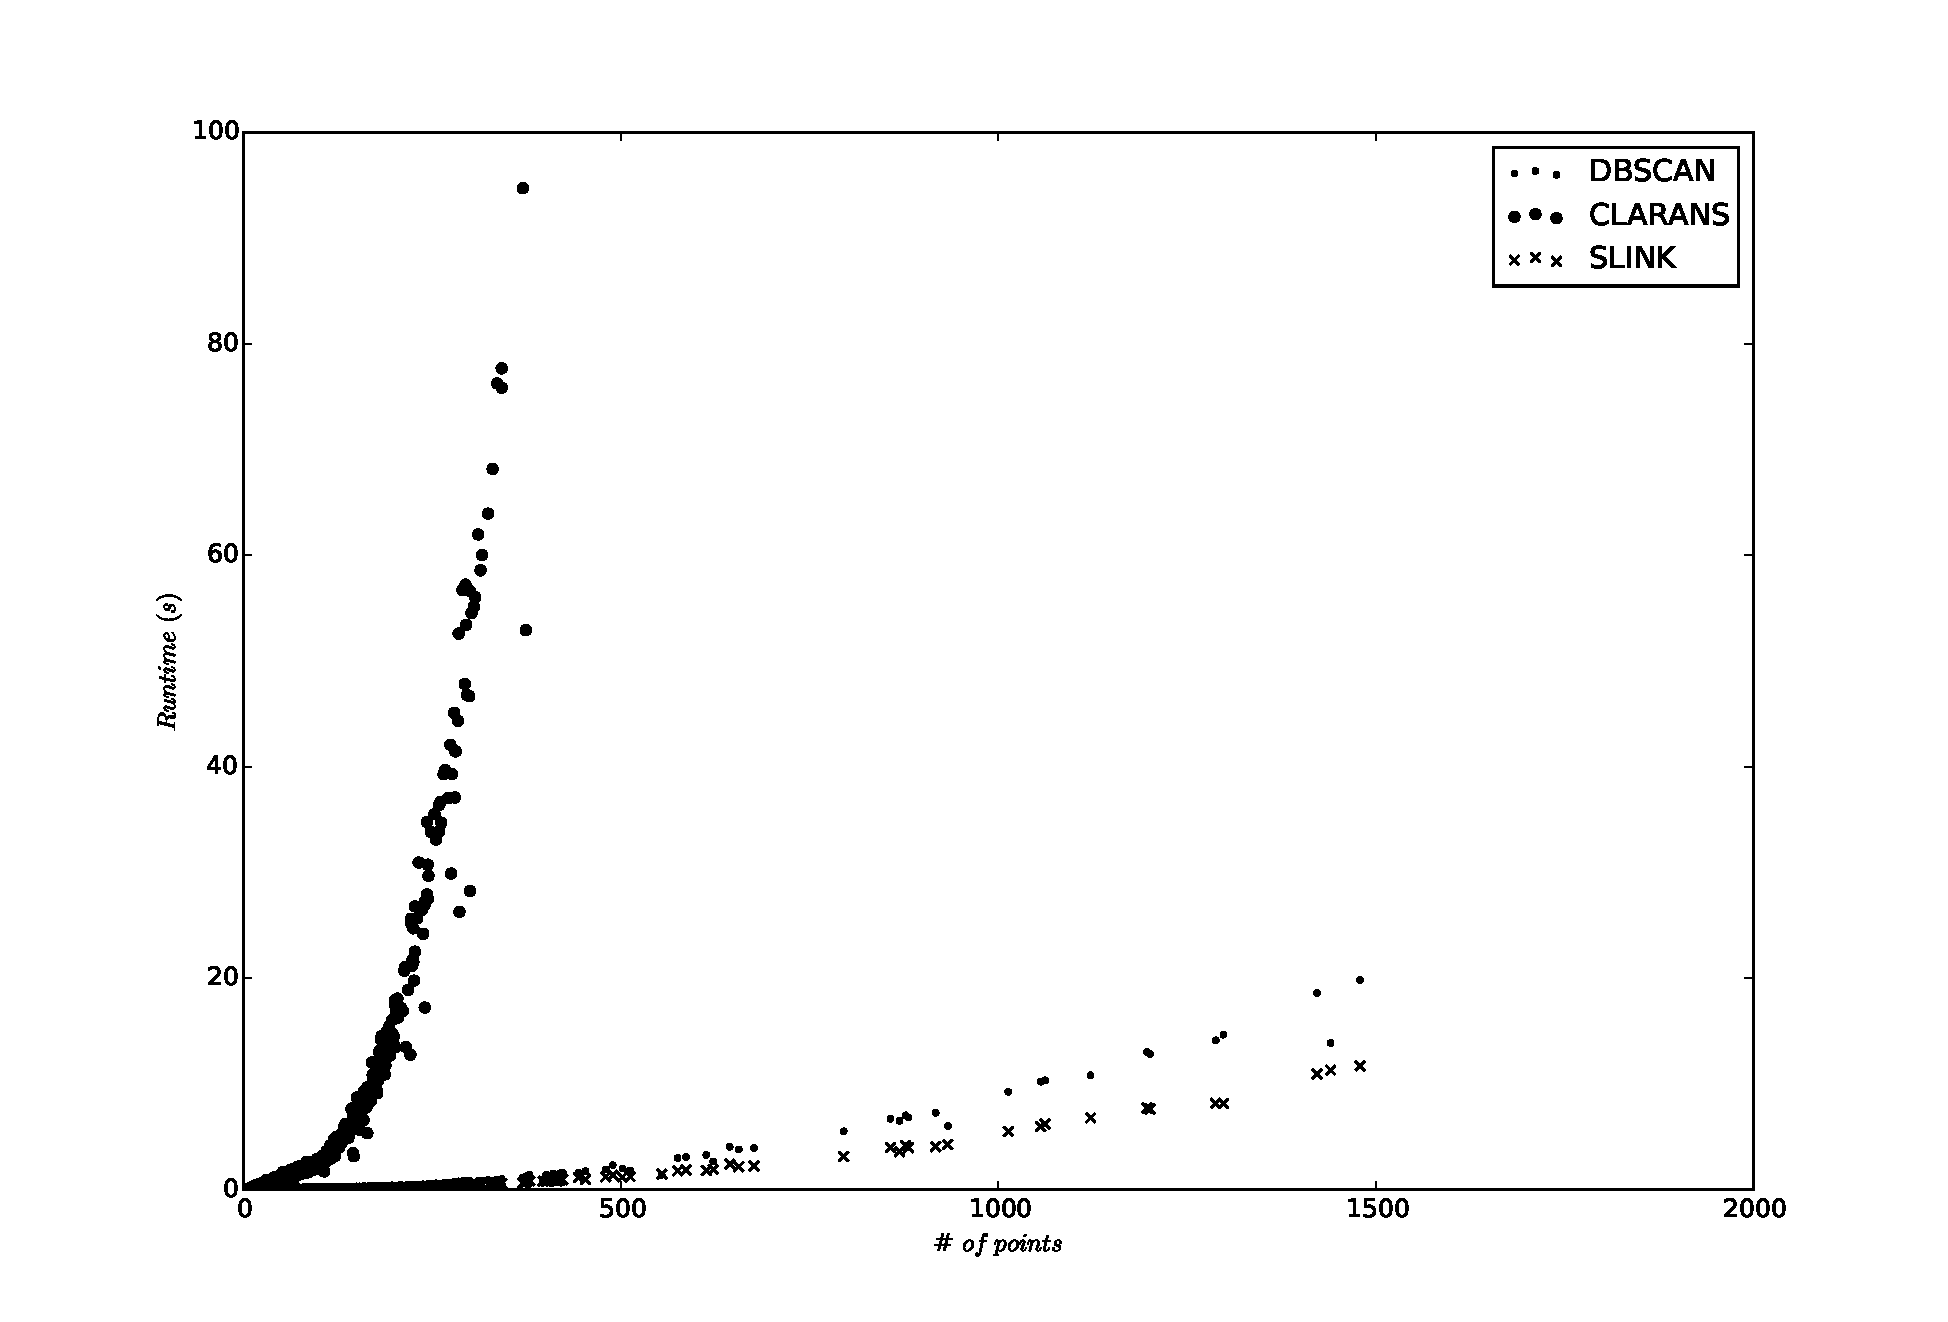
\includegraphics[width=0.9\textwidth]{plots/moment_runtime_scatter.pdf}
    \repeatcaption{fig:moment-runtime-scatter}{
        Run-time for clustering algorithms over Moments, by number of points in the moment.}
\end{sidewaysfigure}

\begin{sidewaysfigure}
    \centering
    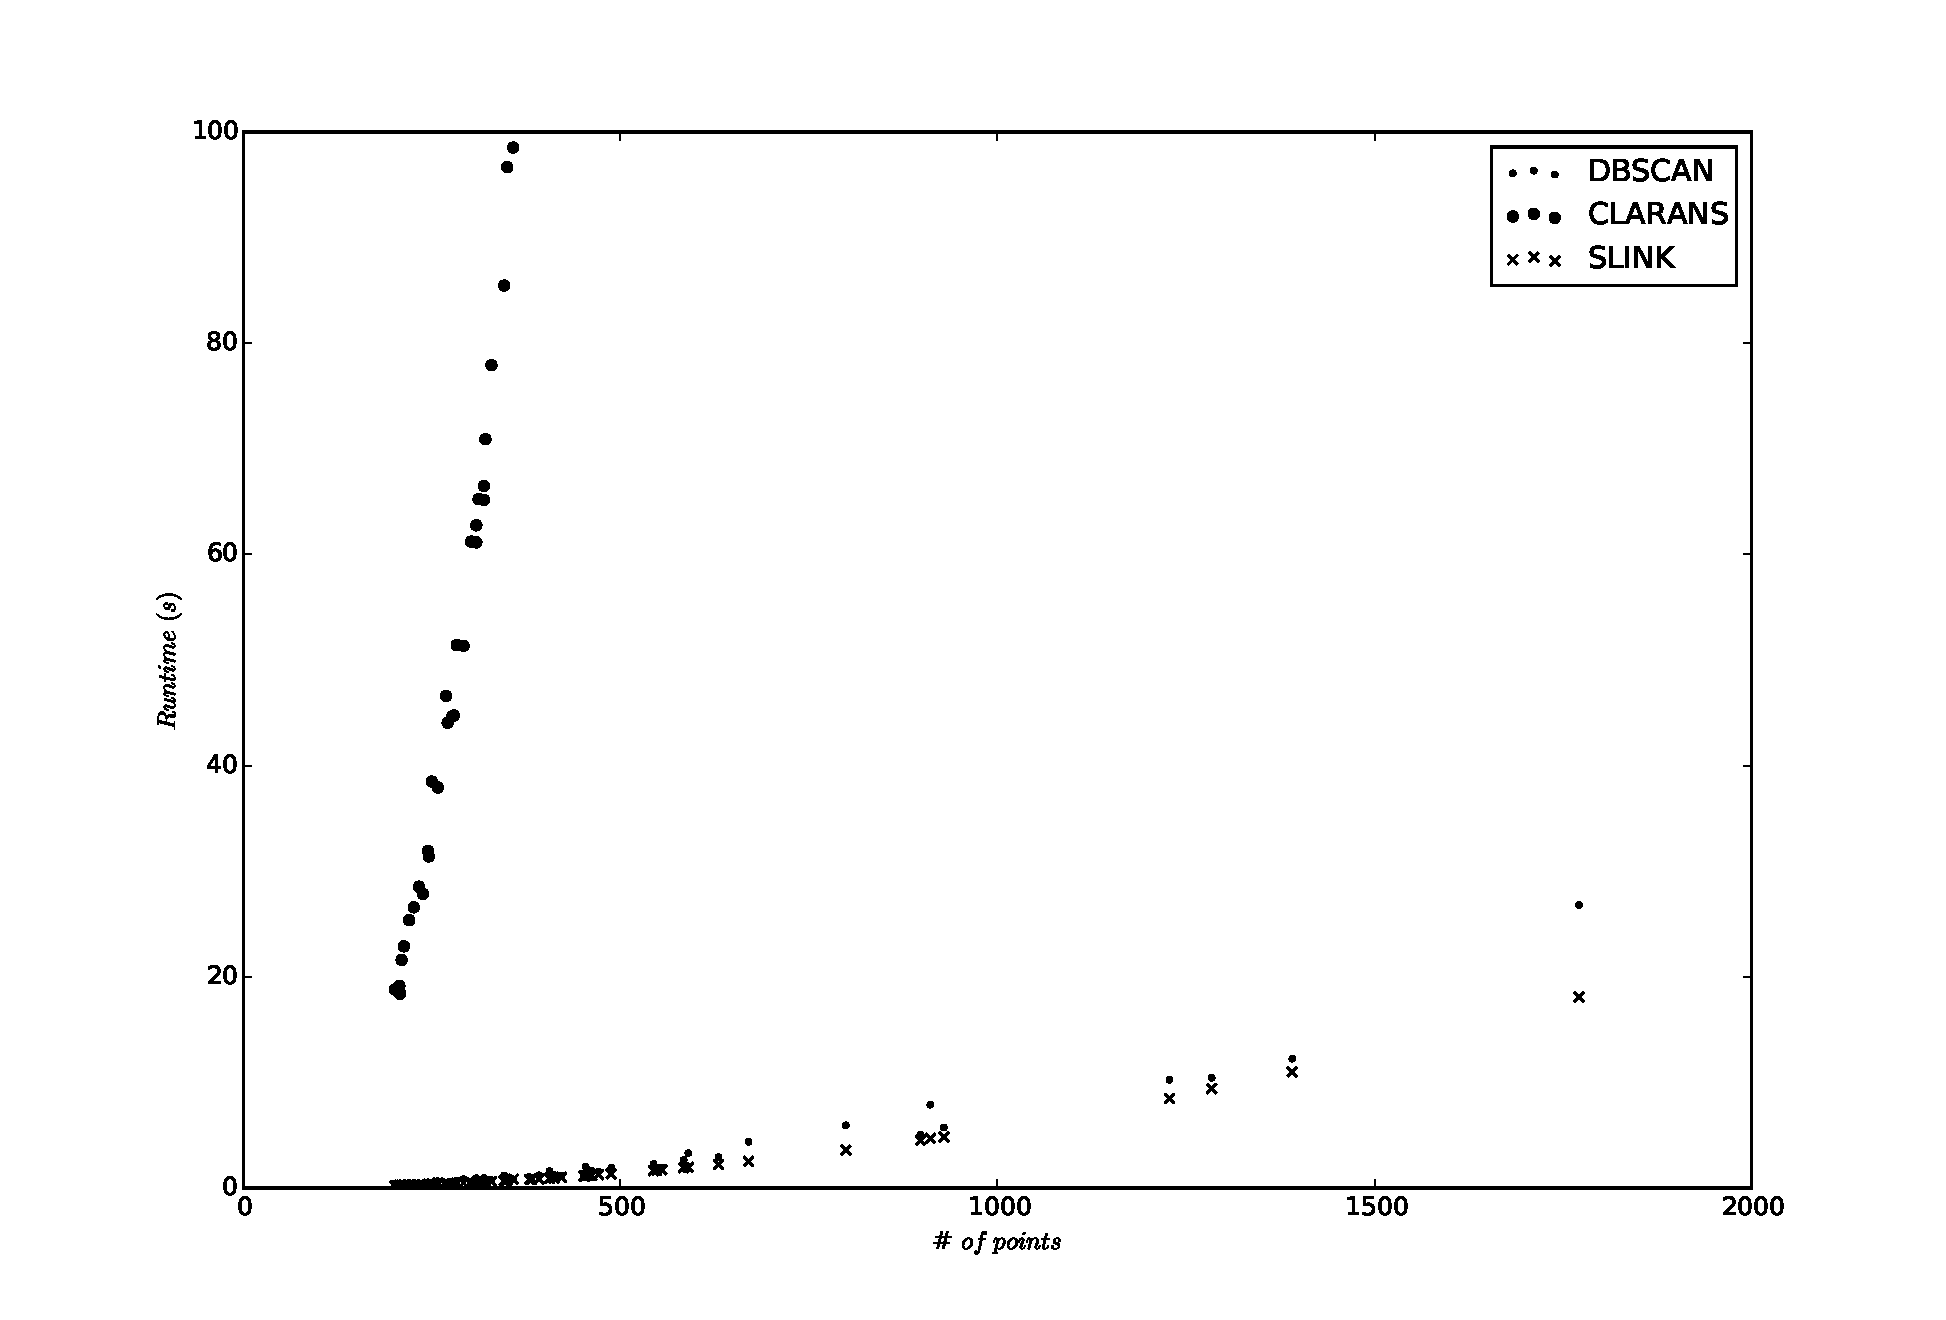
\includegraphics[width=0.7\textwidth]{plots/days_runtime_scatter.pdf}
    \repeatcaption{fig:day-runtime-scatter}
    {Run-time for clustering algorithms over users days, by number of points on the day. }
\end{sidewaysfigure}

\begin{sidewaysfigure}
    \centering
    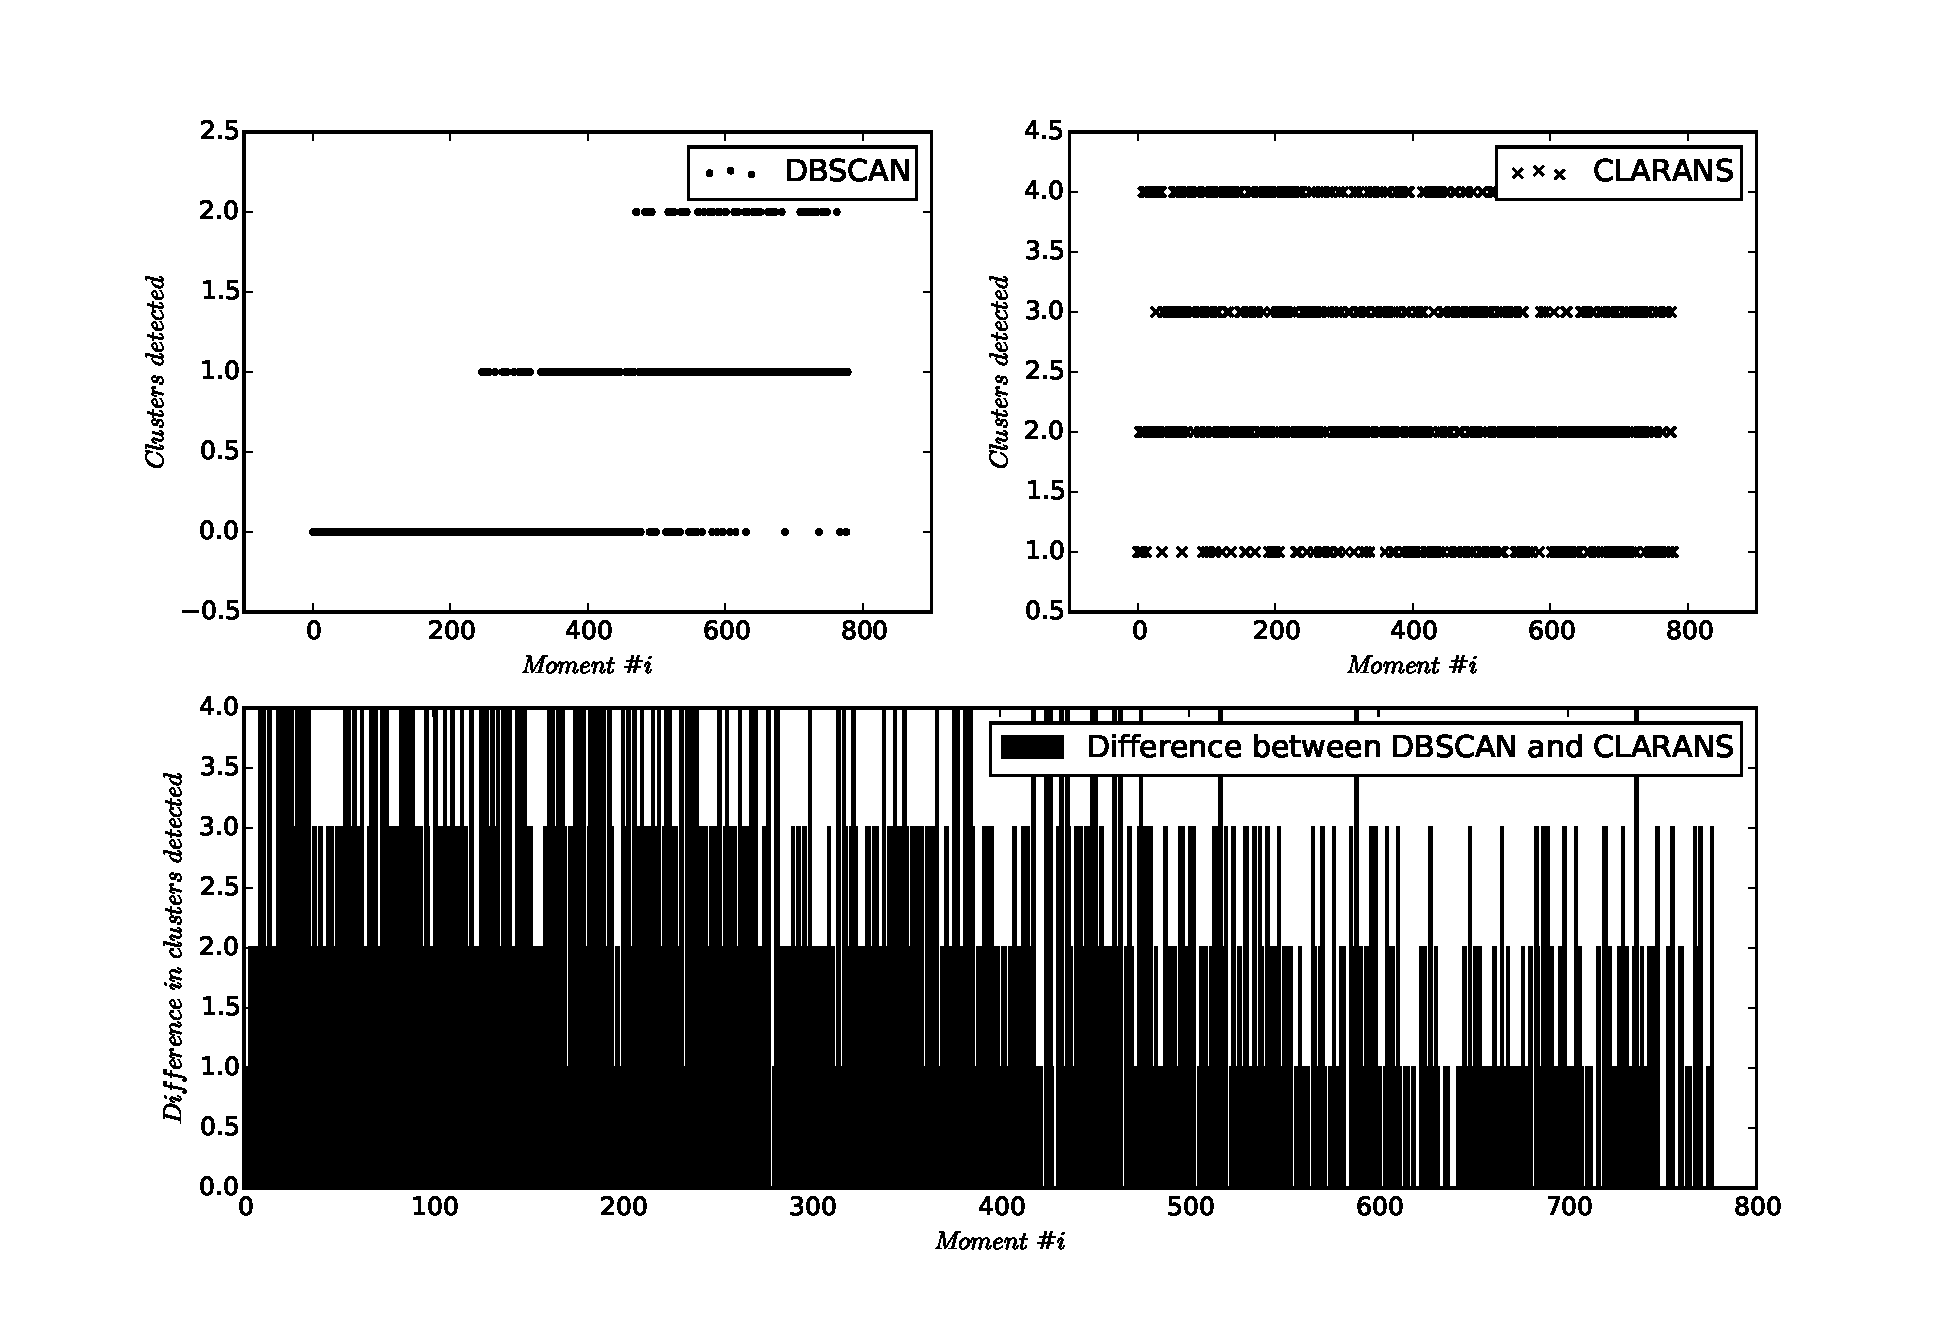
\includegraphics[width=0.9\textwidth]{plots/dbscan_vs_clarans.pdf}
    \repeatcaption{fig:dbscan-vs-clarans}
    {Cluster detection, comparison between DBSCAN and CLARANS. }
\end{sidewaysfigure}

\begin{sidewaysfigure}
    \centering
    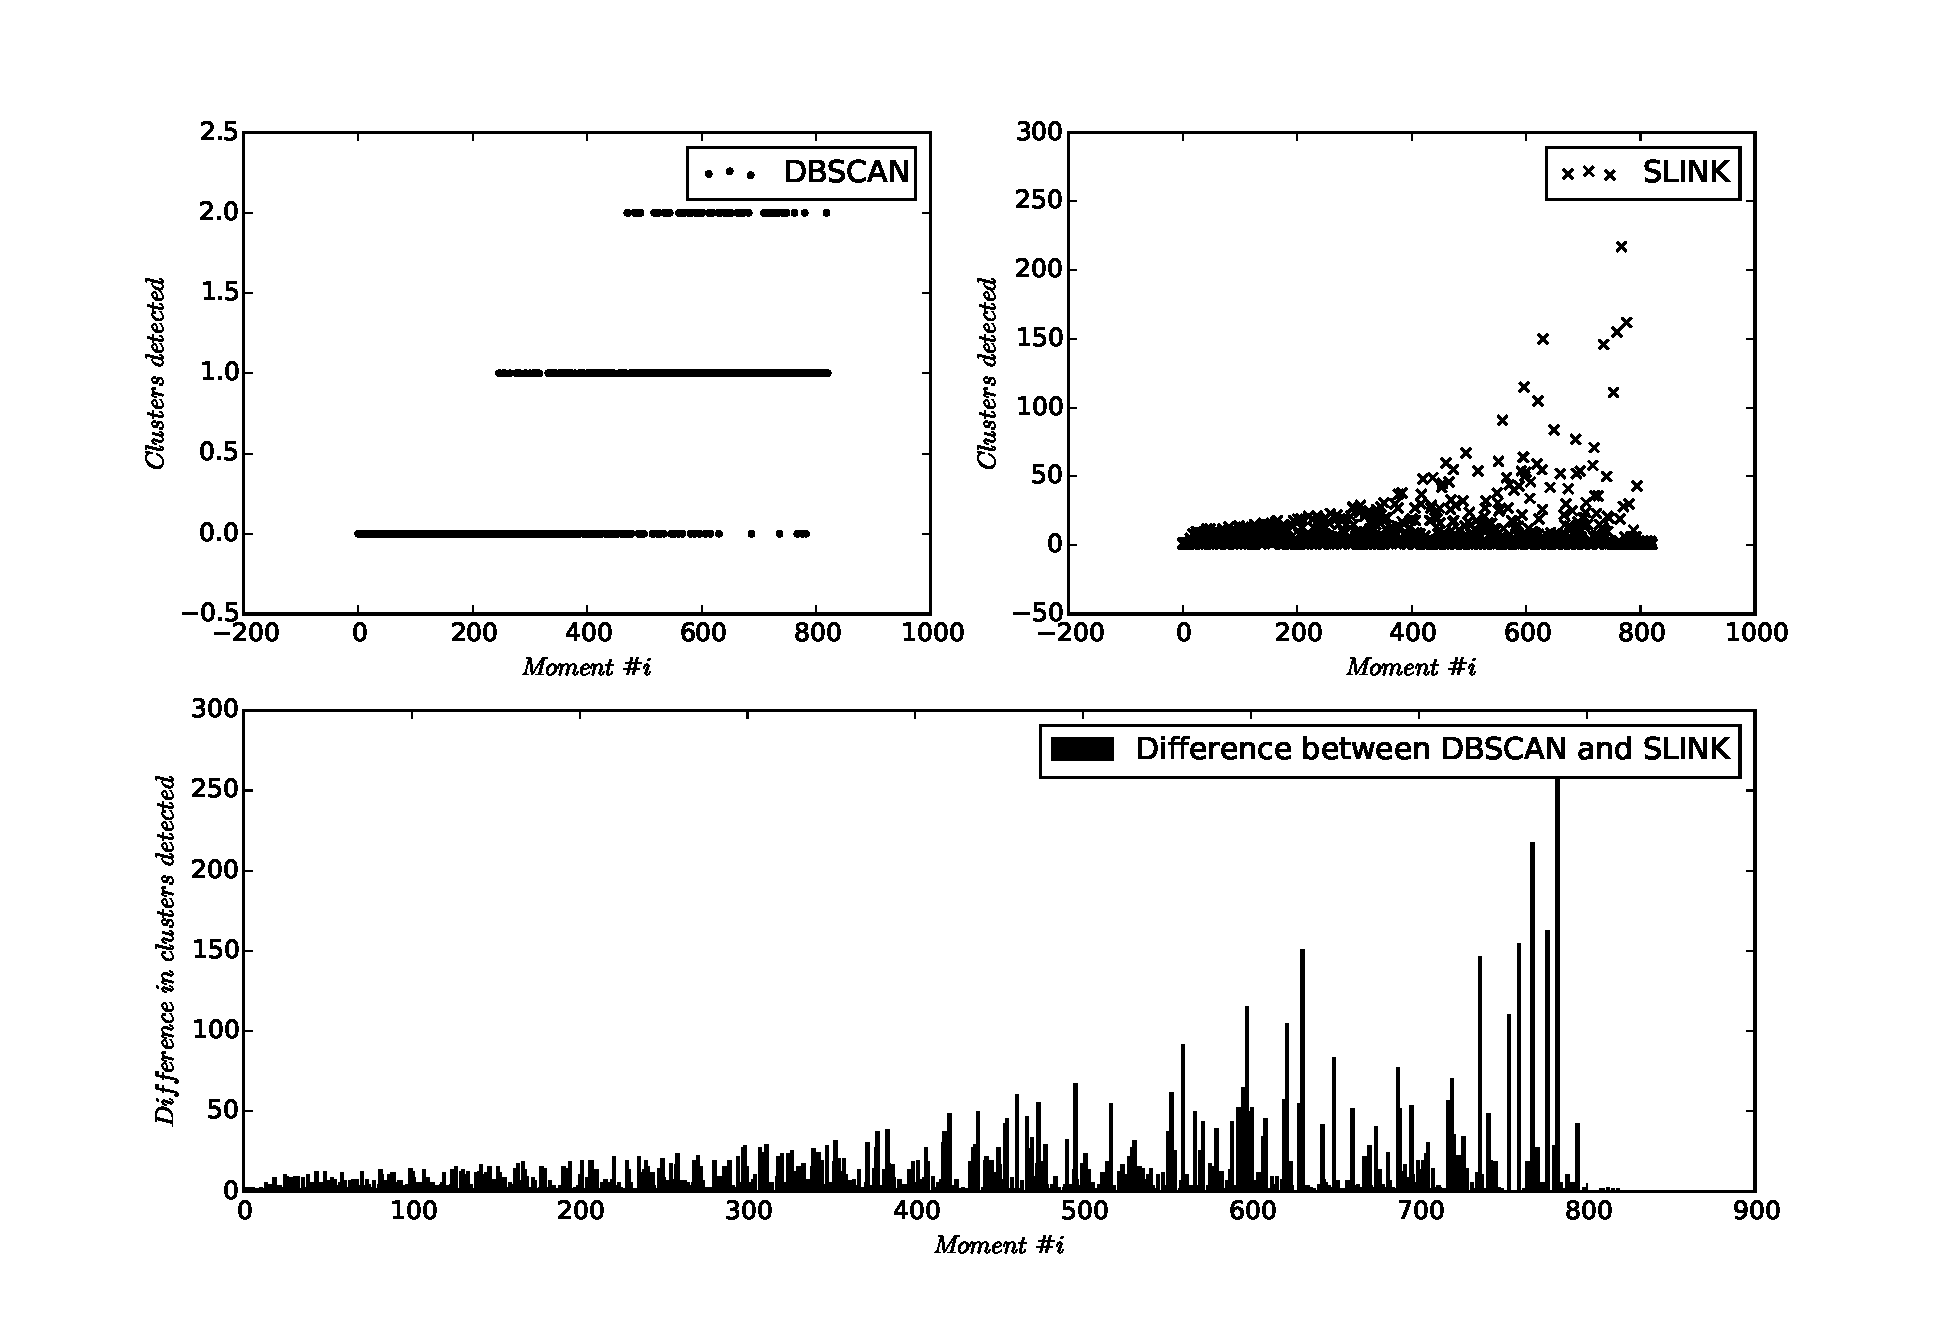
\includegraphics[width=0.9\textwidth]{plots/dbscan_vs_slink.pdf}
    \repeatcaption{fig:dbscan-vs-slink}
    {Cluster detection, comparison between DBSCAN and SLINK. }
\end{sidewaysfigure}

\begin{sidewaysfigure}
    \centering
    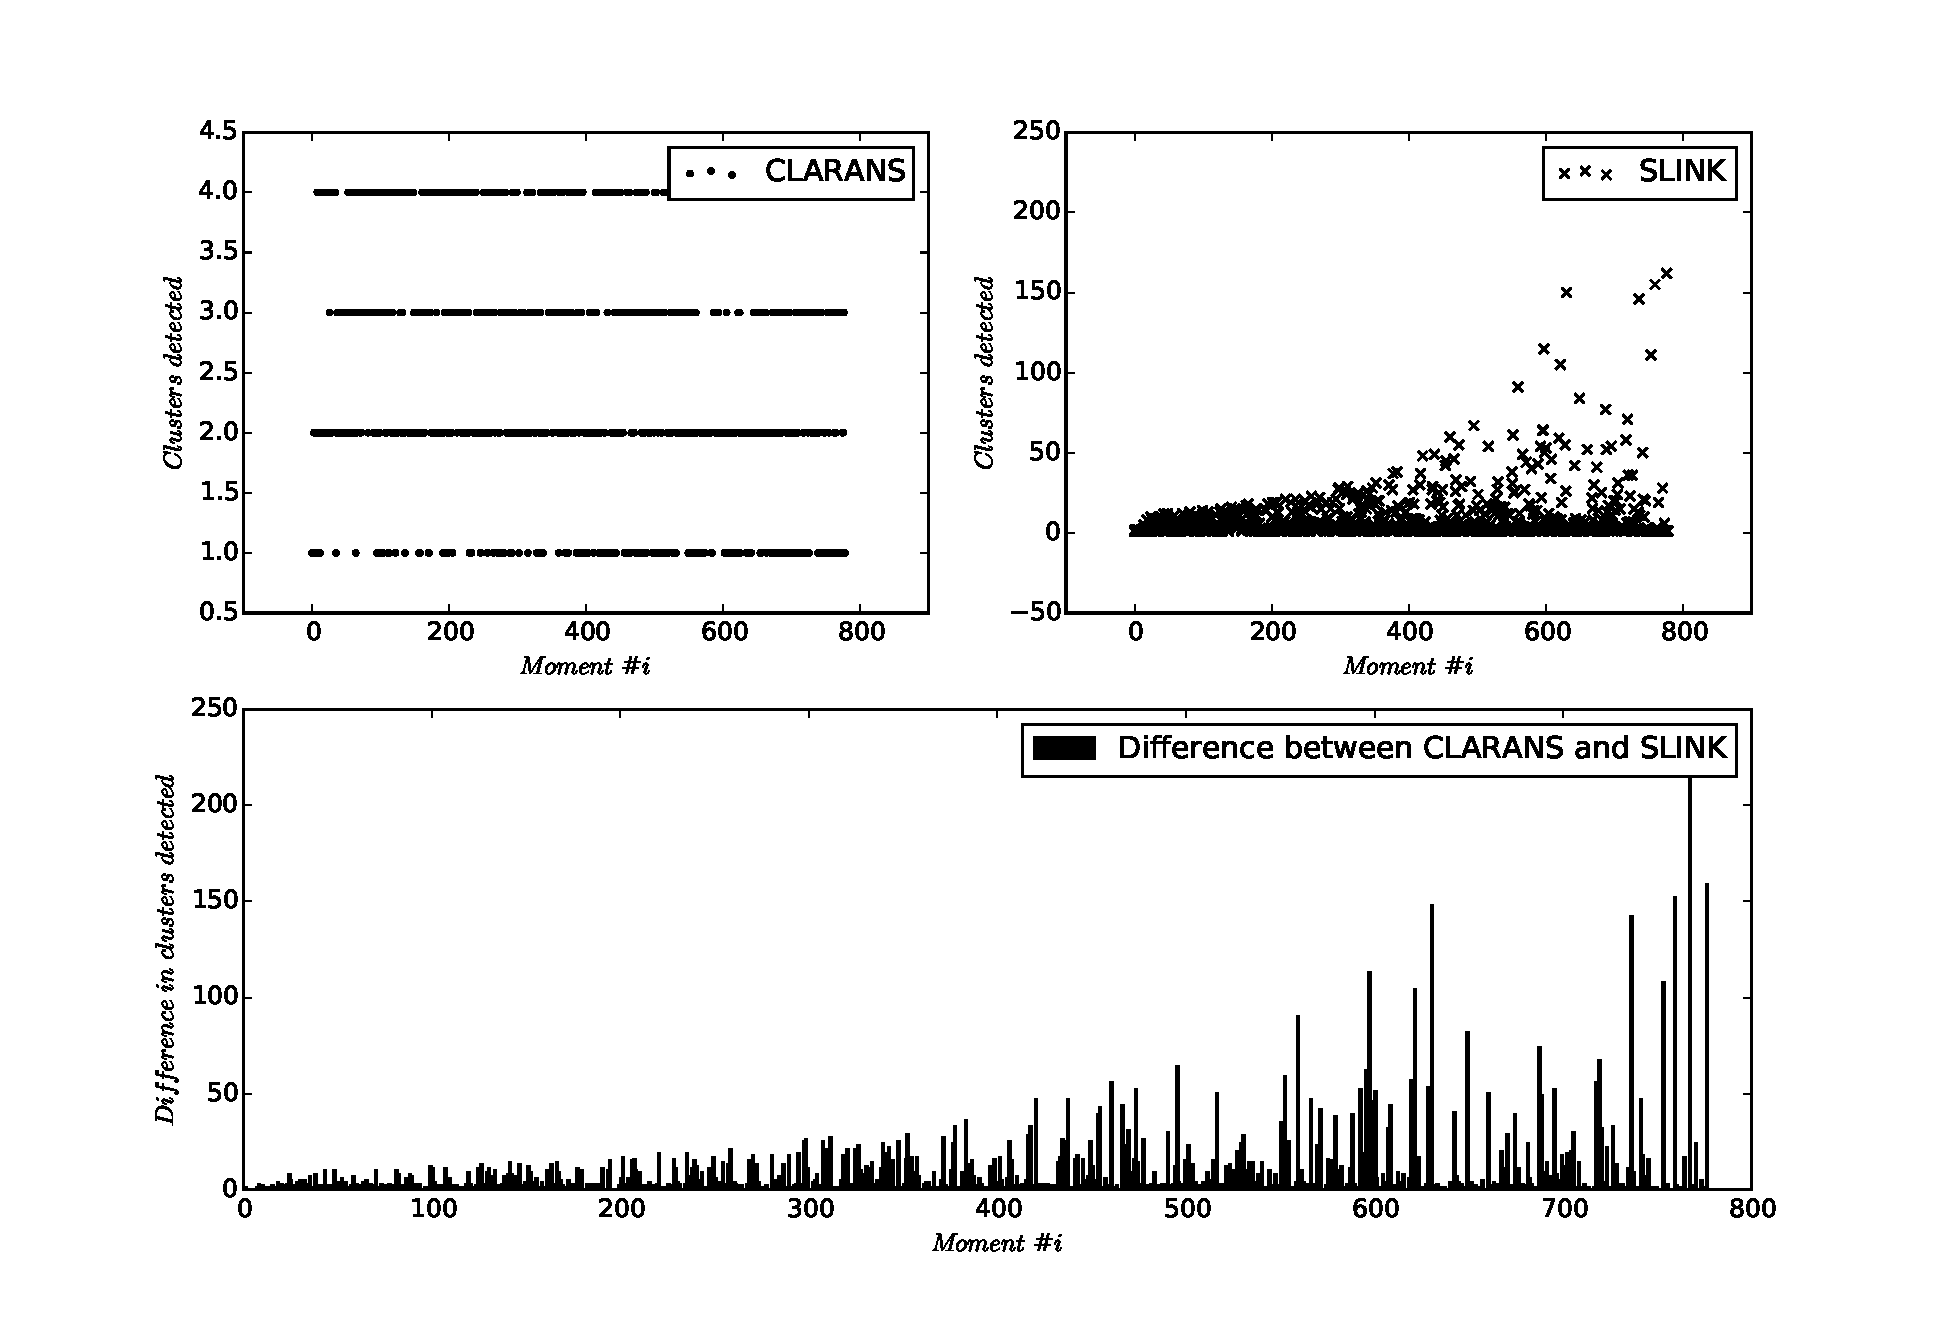
\includegraphics[width=0.9\textwidth]{plots/clarans_vs_slink.pdf}
    \repeatcaption{fig:clarans-vs-slink}
    {Cluster detection, comparison between CLARANS and SLINK. }
\end{sidewaysfigure}

\begin{sidewaysfigure}
    \centering
    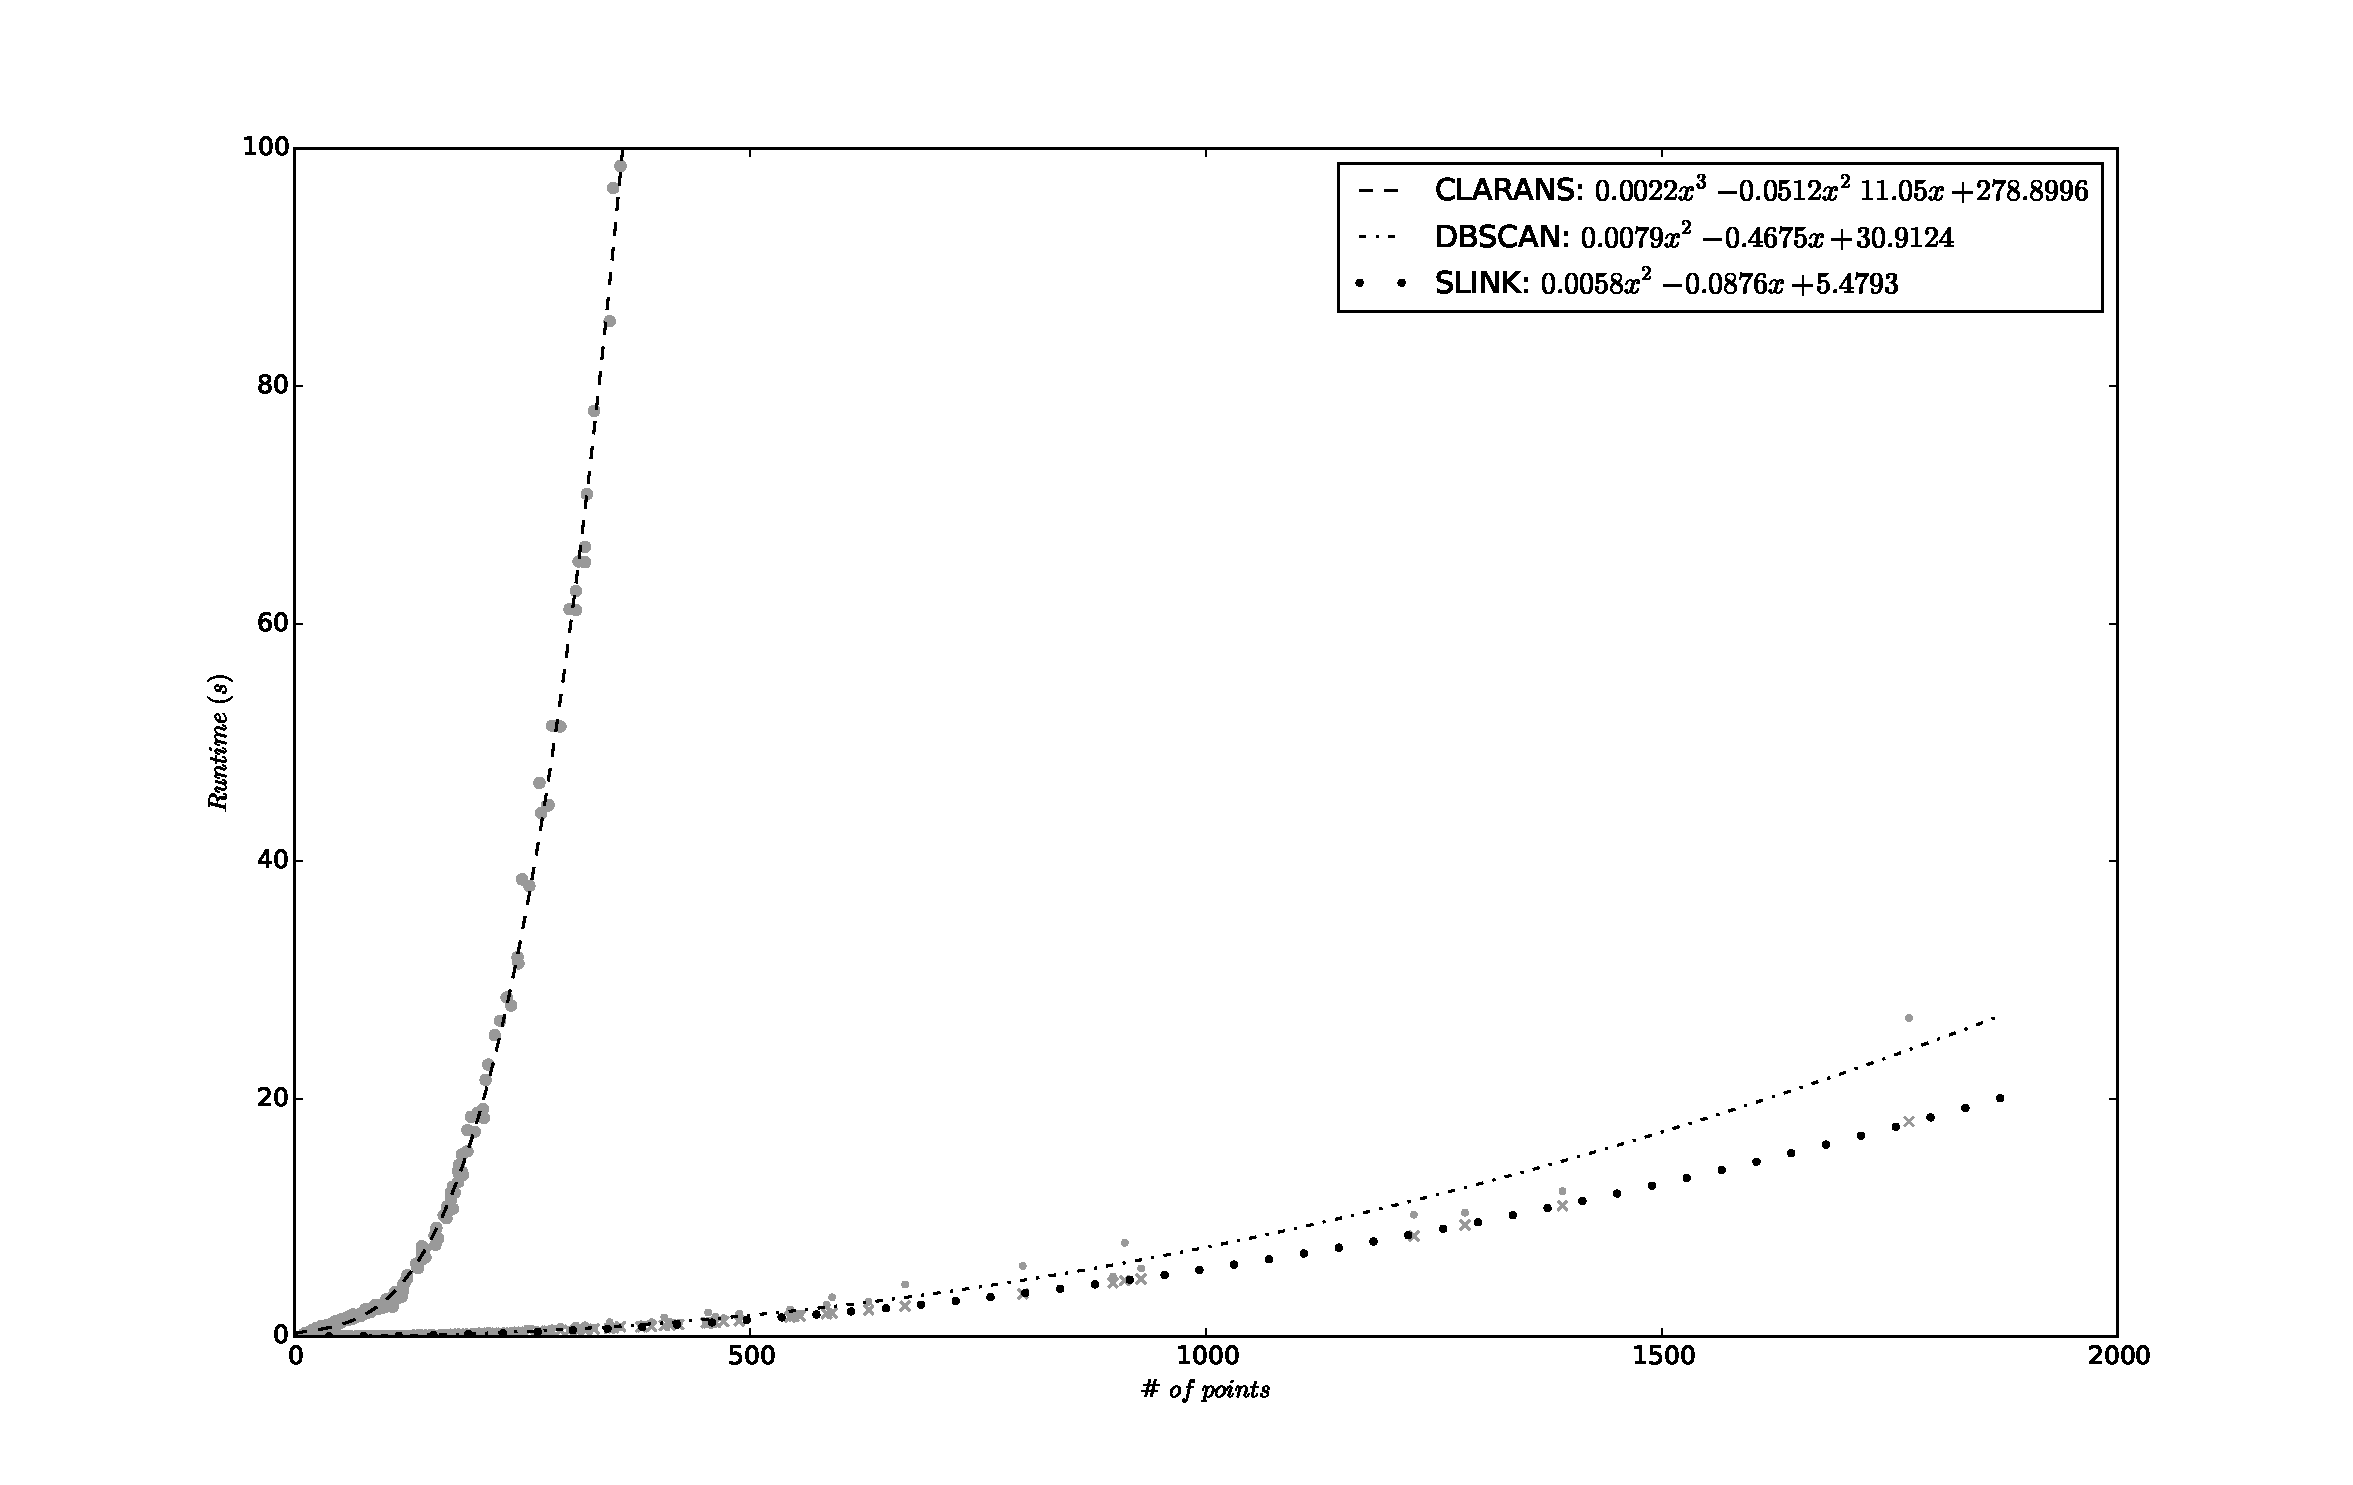
\includegraphics[width=0.9\textwidth]{plots/time_trendlines.pdf}
    \repeatcaption{fig:time-trendlines}{Scatterplot of timestamps including trend lines.}
\end{sidewaysfigure}